\section{Results}

\subsection{Second-Order Differentiators with Large NA, High Transmission, and Broadband Operation}

This second-order benchmark is emphasized here because it simultaneously requires large numerical aperture, high transmission, broadband operation, response curvature control, center suppression, outer-angle support, and practical image-processing behavior. The verified second-order score is evaluated wavelength by wavelength on the $T_{pp}$ response row. The resulting score landscape is highly nonuniform, with mean scores around $0.15$--$0.17$ over the full dataset but top candidates rising above $0.93$ at 1050 and 1100~nm. This gap is important: it shows that the feasible set is sparse but not empty, exactly the regime in which generative candidate exploration is valuable.

At 1050 and 1100~nm, the top verified second-order candidates both reach scores slightly above $0.93$, and a second high-quality family is also visible near 1150~nm with scores above $0.925$. These leading devices were not selected for one isolated metric. They are highlighted because they jointly exhibit the operator-like bowl around $\theta=0$, strong growth toward large $|\theta|$, and robust amplitude at high angles.

\begin{figure}[!htbp]
\centering
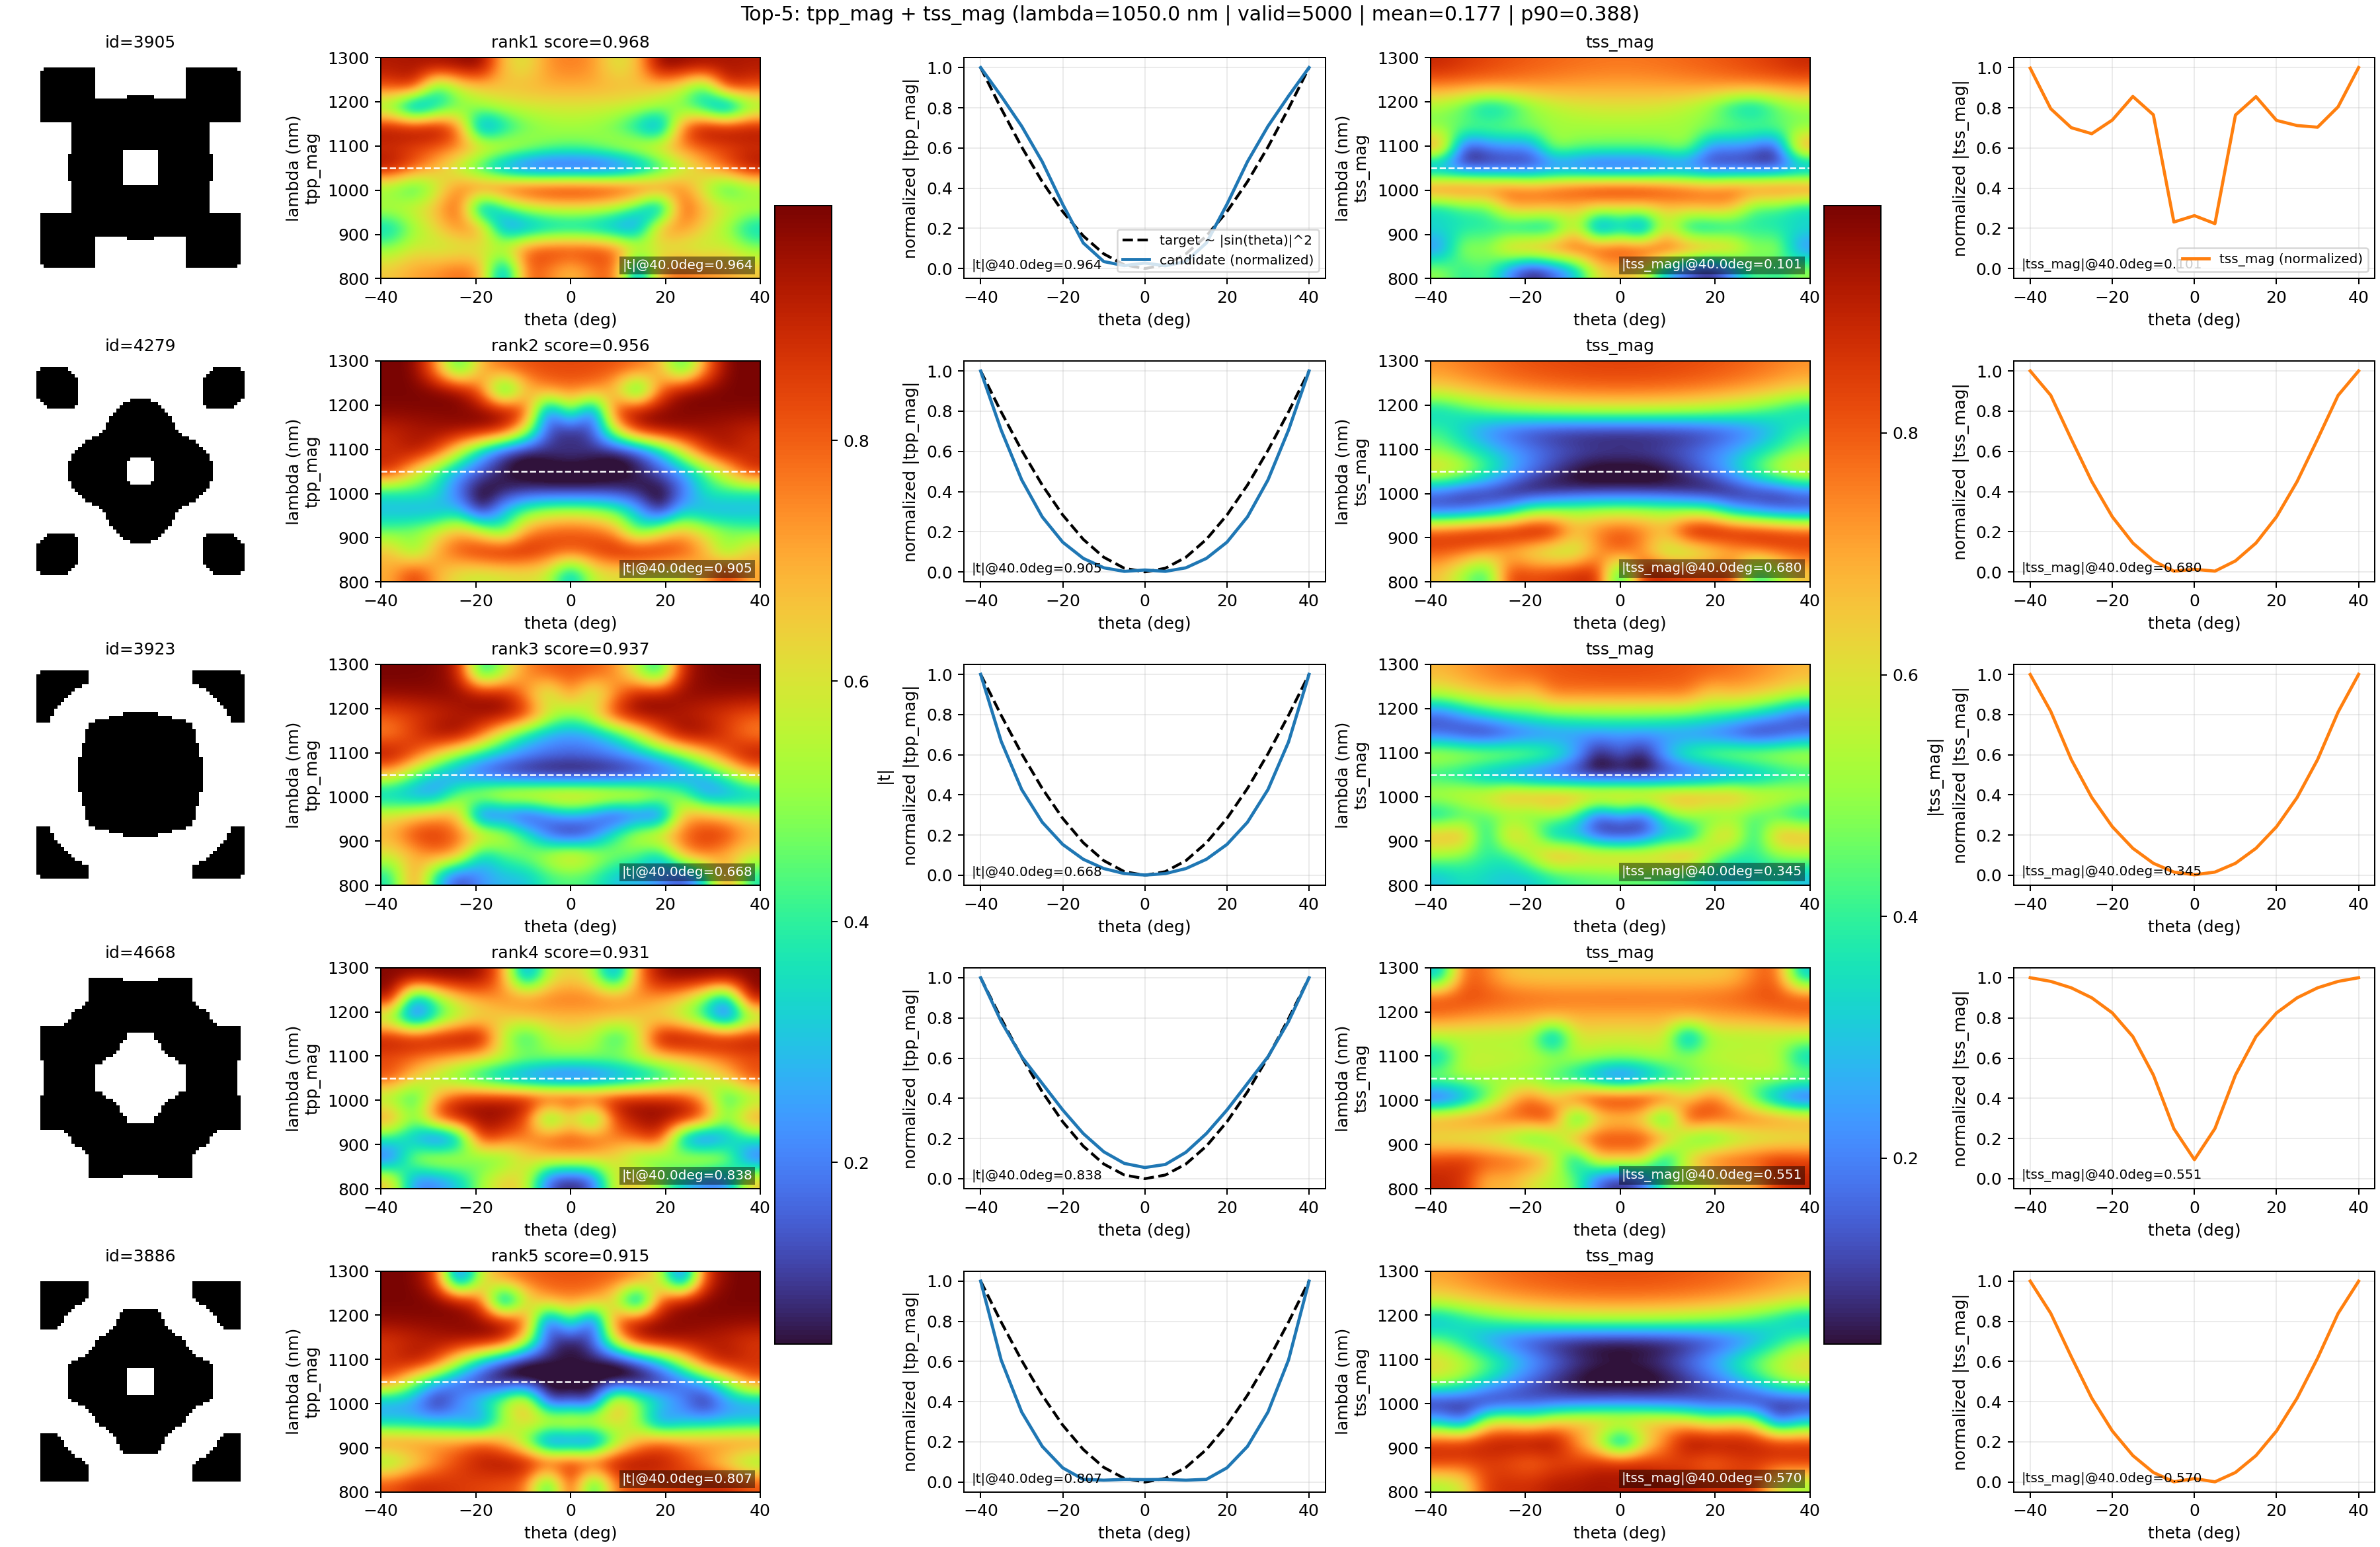
\includegraphics[width=0.78\linewidth]{../data/second_order_scores/tpp_mag_top5_plots/lambda_1050.0nm_top5.png}
\caption{Top ranked second-order candidates at 1050~nm. The ranking overview visualizes the concentration of operator-like responses that motivates task-aware simulation-based reranking.}
\label{fig:second1050}
\end{figure}

Figure~\ref{fig:second1050} shows the top-five ranking overview at 1050~nm, where the leading candidate already displays a representative second-order response. The result is more than a ``high score by normalization.'' It preserves the expected second-order envelope over a wide angular aperture and therefore remains meaningful under operator-level interpretation. The recurrence of closely related high-performing responses across independent evaluations suggests that the best second-order devices occupy especially stable regions of the verified response manifold.

The second-order case also supports the strongest literature-level positioning. Under the same downstream imaging analysis used throughout this study, the best 1050~nm result is associated with a normalized task score of about $0.988$, a relative edge amplitude ratio near $0.97$, an effective working bandwidth around $100$~nm, and a numerical aperture around $0.64$. These numbers place the design in the same performance conversation as recent broadband, high-NA, high-efficiency differentiator reports \cite{cotrufo2023natcom,deng2024,qiu2025highorder,zhou2025laplace}. The precise contribution of the present work, however, is different from a single-device record chase: the same response-centered framework produces this high-performing second-order behavior and also extends naturally to polarization and spatiotemporal targets.

\begin{figure}[!htbp]
\centering
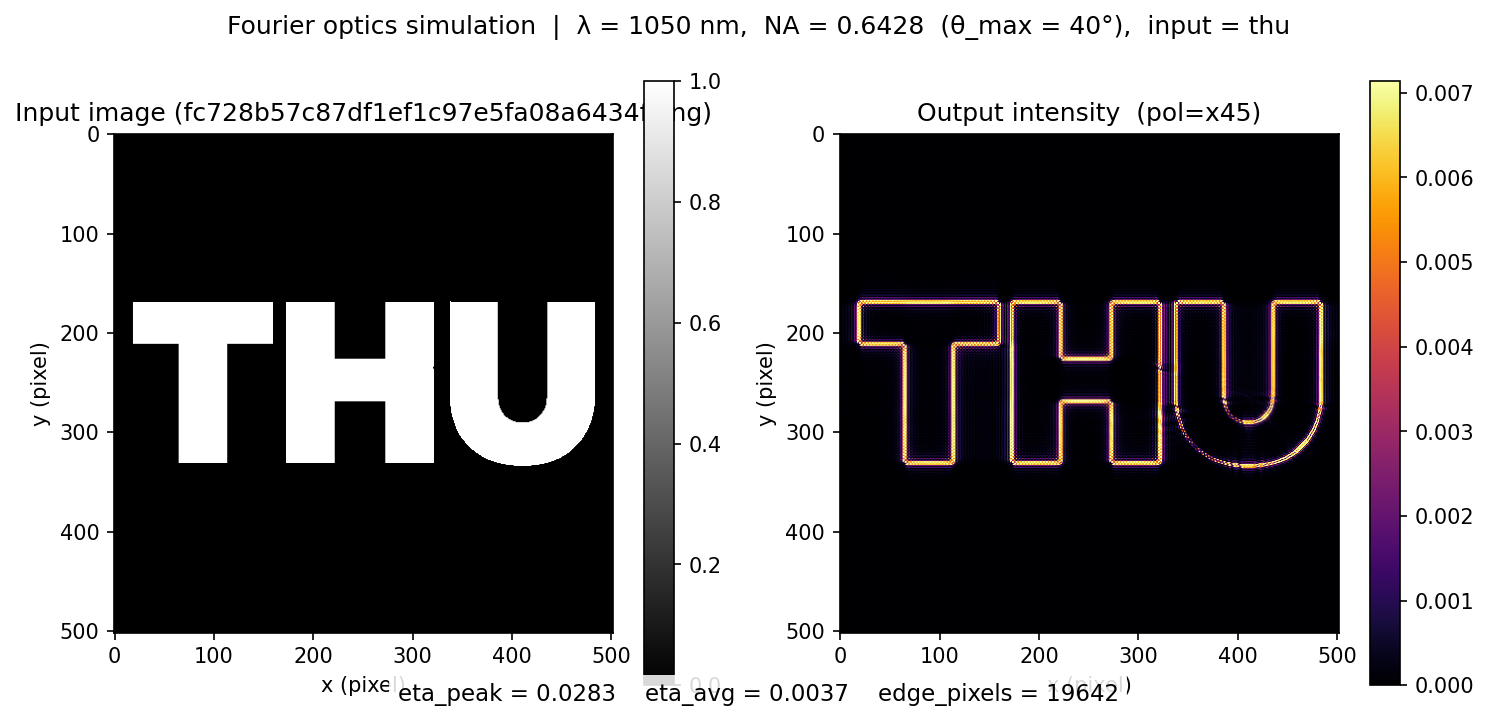
\includegraphics[width=0.63\linewidth]{../src/infer/results/p/1050nm_id4279/run_imaging_p_1050nm_id4279_1050nm_from_kspace_x45_thu_20260405_162600/imaging_result.png}
\caption{Image-domain validation for the leading 1050~nm second-order result. The response-level agreement translates into practical edge-enhancement behavior rather than remaining a numerical score gain only.}
\label{fig:imaging}
\end{figure}

Figure~\ref{fig:imaging} closes the argument by moving from response space to image space. Once the verified transfer function is inserted back into the Fourier imaging pipeline, the resulting output exhibits the expected second-derivative effect: low-frequency regions are suppressed while edge-like features and curvature-sensitive structures are enhanced. This is the key bridge between operator scoring and practical device function. The inverse-design loop is successful because a physically verified structure reproduces both the target response geometry and its intended optical action.

\begin{table}[!htbp]
\centering
\caption{Representative verified results used throughout the paper. Scores reflect task-specific rankings rather than abstract model confidence.}
\label{tab:cases}
\begin{tabular}{>{\raggedright\arraybackslash}p{3.3cm}c>{\raggedleft\arraybackslash}p{2.2cm}>{\raggedleft\arraybackslash}p{4.1cm}}
\toprule
Task & $\lambda$ (nm) & Main score & Notes \\
\midrule
Second-order & 1050 & 0.9306 & representative $T_{pp}$ response with large NA and high transmission \\
Second-order & 1100 & 0.9308 & strongest verified 1100~nm result \\
Polarization independent & 1000 & 0.9358 & matched dual-channel operator response \\
Polarization multiplexed & 1100 & 0.7283 & active score $0.9348$ with passive suppression retained \\
Fourth-order & 1150 & 0.8884 & sharp outer-angle growth \\
Low-pass & 1050 & 0.9934 & strongest passband-shaping result \\
Spatiotemporal window & 950 & 0.7271 & strongest merged window score in the verified screen \\
\bottomrule
\end{tabular}
\end{table}

\FloatBarrier

\subsection{Generalization to other OTF targets}

The most important question after this second-order result is whether the same response-centered loop continues to behave coherently when the target shape changes. The verified results give a positive answer across three independent axes.

The first axis is polarization. In the polarization-independent benchmark, the best 1000~nm result reaches a joint verified score of $0.9358$, while the leading 1050 and 1100~nm results remain above $0.88$ and $0.91$, respectively. This matters because the task score does not merely average two channels: it rewards channel-wise operator fidelity and explicit amplitude agreement around $\pm40^{\circ}$. The fact that the same framework can produce matched $T_{pp}$ and $T_{ss}$ operator responses shows that polarization enters naturally as a first-class conditioning axis.

The second axis is polarization multiplexing. The strongest verified multiplexed result at 1100~nm reaches a joint score of $0.7283$, together with an active-channel operator score of $0.9348$ and a passive-channel suppression term of $0.5218$. In other words, the framework learns to preserve operator shape while also distinguishing which channel should carry the response and which should remain as silent as possible. This is exactly the kind of channel-level tradeoff that a unified response tensor should expose.

\begin{figure}[!htbp]
\centering
\begin{minipage}[t]{0.48\linewidth}
\centering
\includegraphics[width=\linewidth]{../data/polarization_independent_scores/joint_top1_plots/lambda_1000.0nm_top1.png}
\end{minipage}\hfill
\begin{minipage}[t]{0.48\linewidth}
\centering
\includegraphics[width=\linewidth]{../data/polarization_multiplexed_scores/p_active_s_silent/p_active_s_silent_top5_plots/p_active_s_silent_lambda_1100.0nm_top5.png}
\end{minipage}
\caption{Polarization-aware generalization. Left: polarization-independent top case at 1000~nm. Right: polarization-multiplexed top candidates at 1100~nm. The same inverse-design loop can either align the two channels or intentionally separate them.}
\label{fig:pol}
\end{figure}

The third axis is target-shape diversity. In the fourth-order benchmark, the 1050~nm response family reaches a top score of $0.9222$, while the strongest verified 1150~nm result reaches $0.8884$. These values indicate that the framework remains effective even when the desired response becomes sharper than a second-order bowl. In the low-pass benchmark, the best verified results reach $0.9934$ at 1050~nm and $0.9863$ at 1100~nm, demonstrating that the same tensor-conditioning strategy can realize a fundamentally different angular envelope in addition to polynomial-like operator responses.

Spatiotemporal targets provide the strongest stress test because they are evaluated on a two-dimensional wavelength--angle window instead of a single wavelength row. The dataset-level screen at 950~nm identifies a top merged score of $0.7271$, which is already meaningful given the difficulty of jointly controlling the central zero lines and the corner lobes of the ideal map. This confirms that the response-window view is not merely rhetorical, but remains quantitatively meaningful under the same verified ranking logic.

\begin{figure}[!htbp]
\centering
\begin{minipage}[t]{0.48\linewidth}
\centering

\includegraphics[width=\linewidth]{../data/optica_lowpass_scores/tpp_mag_optica_lowpass_top5_plots/lambda_1050.0nm_top5.png}
\end{minipage}\hfill
\begin{minipage}[t]{0.48\linewidth}
\centering
\includegraphics[width=\linewidth]{../data/st2_template_match_20260330_233804/lambda_950nm/rank_001_sample_5409.png}
\end{minipage}
\caption{Generalization beyond second-order differentiation. Left: low-pass target at 1050~nm. Right: top spatiotemporal candidate at 950~nm from the wavelength--angle window ranking pipeline.}
\label{fig:generalization}
\end{figure}

Taken together, Figures~\ref{fig:pol} and~\ref{fig:generalization} support the same conclusion. The present method goes beyond a differentiator-specific recipe. It forms a unified response-space design loop that can absorb changes in channel requirements, target curvature, target envelope, and even in the dimensionality of the target support.

\FloatBarrier

\subsection{Model comparison and evaluation protocol}

A unified comparison protocol is defined for topology optimization, CVAE, cGAN, and diffusion under the same target condition and the same simulation-based post-verification metrics. The shared evaluation reports best score, mean score, top-3 score, success rate above threshold, spectrum MAE, binary rate, diversity, and inference time. This is the correct comparison language for the present problem because a strong inverse designer should hit good samples consistently and should also populate the feasible set with diverse physically useful candidates.

At the current stage of the study, the retained checkpoints directly support the forward surrogate and the physics-guided diffusion pipeline, whereas the cVAE and cGAN baselines and the topology-optimization branch are not all accompanied by synchronized checkpoints. Table~\ref{tab:compare} therefore serves two purposes. It makes the quantitative protocol explicit and it records only the directly available evidence without fabricating missing baseline numbers.

\begin{table}[!htbp]
\centering
\caption{Comparison protocol used in this study. The metrics are computed after full-wave verification. Quantitative training endpoints are listed only where directly retained evidence is available.}
\label{tab:compare}
\begin{tabular}{>{\raggedright\arraybackslash}p{2.1cm}>{\raggedright\arraybackslash}p{2.4cm}>{\raggedleft\arraybackslash}p{2.1cm}>{\raggedleft\arraybackslash}p{2.1cm}}
\toprule
Method & Condition / objective & Direct retained evidence & Status \\
\midrule
Forward surrogate & structure $\rightarrow$ response, normalized $L_1$ & val loss $\approx 0.366$ & checkpoint + log retained \\
Diffusion & response $\rightarrow$ structure, diffusion + physics + binary losses & val loss $\approx 0.129$ & checkpoint + log retained \\
CVAE & response $\rightarrow$ structure, variational baseline & unified eval supported & checkpoint absent locally \\
cGAN & response $\rightarrow$ structure, adversarial baseline & unified eval supported & checkpoint absent locally \\
Topo-opt & task-guided iterative search & unified eval supported & legacy dependency incomplete locally \\
\bottomrule
\end{tabular}
\end{table}

Even with this limitation, the comparison section remains scientifically useful. The evaluation protocol already formalizes the right question: the inverse method should be judged by verified best-case score, average candidate quality, response MAE, binarity, and diversity under shared targets. The present physics-guided diffusion pipeline is the only branch for which the end-to-end checkpointed evidence is directly retained, which is why it becomes the center of the manuscript.
